% \documentclass{beamer}
% \documentclass[aspectratio=169]{beamer}
\documentclass[aspectratio=169, 11pt, handout]{beamer}
\usetheme{boxes}
% \usecolortheme{beaver}

% \renewcommand{\familydefault}{\sfdefault}

% To get numbers in reference list
% \setbeamertemplate{bibliography item}{\insertbiblabel}

\usepackage{graphicx}
\graphicspath{{images/}}


% \newtheorem{theorem}{Theorem}
%\newtheorem{lemma}{Lemma}
%\newtheorem{problem}{Problem}
%\newtheorem{definition}{Definition}
%\newtheorem{corollary}{Corollary}

\renewcommand{\baselinestretch}{1.1} 
\setlength{\parskip}{\bigskipamount}

% \usepackage{biblatex}
% \usepackage[numbers]{natbib}
\usepackage{tikz}
\usetikzlibrary{tikzmark,fit,shapes.geometric,arrows,arrows.meta}
\usetikzlibrary{trees}
\usepackage{pgfplots}

\usepackage{wrapfig}
\usepackage[english]{babel}
\usepackage{bbm}
% or whatever
\usepackage[latin1]{inputenc}
% or whatever
\usepackage{times}
\usepackage{bm}
\usepackage[T1]{fontenc}
% Or whatever. Note that the encoding and the font should match. If T1
% does not look nice, try deleting the line with the fontenc.

\usepackage{bibentry}
\usepackage{algorithm, setspace}
%\usepackage[noend]{algorithmic}
\usepackage{algpseudocode}

\usepackage{array}
\usepackage{amsmath}
\usepackage{xspace}
\usepackage{dsfont}
% \usepackage{tocloft}
% \setlength{\cftbeforesecskip}{10pt}
\usepackage{booktabs} % For nice tables

\usetikzlibrary{shadows}
\usetikzlibrary{positioning}
\usepackage{xcolor}
\usepackage[framemethod=TikZ]{mdframed}
\usepackage{tkz-berge,float}
\usepackage{makecell}
\usepackage{amsmath,amssymb}

\usepackage{booktabs} % For formal tables
\usepackage{graphicx}
\usepackage{adjustbox}
\usepackage{epsfig}

\usepackage{url}
\usepackage{hyperref}
\usepackage{tikz}
\usetikzlibrary{shadows}
\usepackage{xcolor}
\usepackage[framemethod=TikZ]{mdframed}
\usepackage{tkz-berge,float}

\usepackage{xargs}
\usepackage{fontawesome}
% \usepgfplotslibrary{external}
% \usetikzlibrary{external}
% \tikzexternalize

% AALTO COLORS
\definecolor{aaltoyellow}{RGB}{254,203,00}  % FECB00
\definecolor{aaltored}{RGB}{237,41,57}      % ED2939
\definecolor{aaltoblue}{RGB}{00,101,189}    % 0065BD
\definecolor{aaltogray}{RGB}{146,139,129}   % 928B81
\definecolor{aaltolgreen}{RGB}{105,190,40}  % 69BE28
\definecolor{aaltodgreen}{RGB}{00,155,58}   % 009B3A
\definecolor{aaltocyan}{RGB}{00,168,180}    % 00A8B4
\definecolor{aaltopurple}{RGB}{102,57,183}  % 6639B7
\definecolor{aaltomagenta}{RGB}{177,05,157} % B1059D
\definecolor{aaltoorange}{RGB}{237,101,00}  % FF7900

% Set caption separation
\setlength{\abovecaptionskip}{3pt plus 3pt minus 2pt}

\newcommand{\txtred}[1]{{\color{aaltored}{#1}}}
\newcommand{\txtblue}[1]{{\color{aaltoblue}{#1}}}
\newcommand{\txtyellow}[1]{{\color{aaltoyellow}{#1}}}
\newcommand{\txtorange}[1]{{\color{aaltoorange}{#1}}}
\newcommand{\txtdgreen}[1]{{\color{aaltodgreen}{#1}}}
\newcommand{\txtgreen}[1]{{\color{aaltolgreen}{#1}}}
\newcommand{\txtmagenta}[1]{{\color{aaltomagenta}{#1}}}
\newcommand{\txtpurple}[1]{{\color{aaltopurple}{#1}}}
\newcommand{\txtgray}[1]{{\color{aaltogray}{#1}}}
\newcommand{\txtcyan}[1]{{\color{aaltocyan}{#1}}}

\newcommand{\hl}[1]{\txtblue{#1}}
\newcommand{\head}[1]{\txtmagenta{#1}}
\newcommand{\colorcite}[1]{{\color{aaltogray}{\cite{#1}}}}
\newcommand{\colorcitet}[1]{{\color{aaltogray}{\citet{#1}}}}
\newcommand{\colorcitep}[1]{{\color{aaltogray}{\citep{#1}}}}

\newcommand{\imgsource}[1]{{\footnotesize \color{aaltogray}{Image source: #1}}}
\newcommand{\inlinecomment}[1]{{\footnotesize \textit{#1}}}

\DeclareMathOperator*{\argmin}{\arg\min}
\DeclareMathOperator*{\argmax}{\arg\max}

\newtheorem{proposition}{Proposition}
\newtheorem{claim}{Claim}
% \newtheorem*{problem*}{Problem}
% \newtheorem*{theorem*}{Theorem}
% \newtheorem*{definition*}{Definition}

\newcommand{\spara}[1]{\smallskip\noindent{\bf{#1}}}
\newcommand{\set}[1]{\left\{#1\right\}}
\newcommand{\abs}[1]{{\left|#1\right|}}
\newcommand{\norm}[1]{\left\lVert#1\right\rVert}
\newcommand{\real}{\ensuremath{\mathbb{R}}\xspace}
\newcommand{\hamming}{\ensuremath{\mathbb{H}}\xspace}
\newcommand{\realnn}{\ensuremath{\real_{\ge 0}}\xspace}
\newcommand{\pr}[1]{\left(#1\right)}
\newcommand{\spr}[1]{\left[#1\right]}
\newcommand{\define}{\leftarrow}

\newcommand{\vw}{\ensuremath{\bm{w}}\xspace}
\newcommand{\mW}{\ensuremath{\bm{W}}\xspace}
\newcommand{\vx}{\ensuremath{\bm{x}}\xspace}
\newcommand{\vy}{\ensuremath{\bm{y}}\xspace}
\newcommand{\vz}{\ensuremath{\bm{z}}\xspace}
\newcommand{\vs}{\ensuremath{\bm{s}}\xspace}
\newcommand{\vh}{\ensuremath{\bm{h}}\xspace}
\newcommand{\vb}{\ensuremath{\bm{b}}\xspace}
\newcommand{\vc}{\ensuremath{\bm{c}}\xspace}

\newcommand{\Xset}{\ensuremath{\mathcal{X}}\xspace}
\newcommand{\Lset}{\ensuremath{\mathcal{L}}\xspace}
\newcommand{\Lpset}{\ensuremath{\mathcal{L}^{'}}\xspace}
\newcommand{\Lp}{\ensuremath{L^{'}}\xspace}
\newcommand{\dbset}{\ensuremath{(\Lset+\Lpset)^H}\xspace}
\newcommand{\simf}{\ensuremath{\text{sim}}\xspace}
\newcommand{\distf}{\ensuremath{d}\xspace}
\newcommand{\simham}{\ensuremath{\simf^H}\xspace}
\newcommand{\dham}{\ensuremath{\distf_H}\xspace}
\newcommand{\sign}{\ensuremath{\text{sgn}}\xspace}
\newcommand{\hamdim}{\ensuremath{K}\xspace}


% \newcommand{\dim}{\ensuremath{d}\xspace}
\newcommand{\Xpos}{\ensuremath{X^{+}}\xspace}
\newcommand{\Xneg}{\ensuremath{X^{-}}\xspace}

\newcommand{\proba}[1]{\ensuremath{\text{Pr}\spr{#1}}\xspace}
\newcommand{\isls}{\ensuremath{\text{ is linearly separable}}\xspace}
\newcommand{\bipart}{\ensuremath{\pr{\Xpos, \Xneg}}\xspace}
\newcommand{\kpart}{\ensuremath{\pr{X_i}_{i=1}^K}\xspace}
\newcommand{\compl}[1]{\ensuremath{\overline{#1}}\xspace}

\newcommand{\indicator}[1]{\ensuremath{\mathbbm{1}\spr{#1}}\xspace}

\newcommand\half{\frac{1}{2}\xspace}
\newcommand\halfn{\pr{\half}^{n}\xspace}
\newcommand{\sectionslide}[1]{
\begin{frame}
\vfill
\begin{center}   
{\large #1}  
\end{center}
\vfill
\end{frame}}


\newcommandx*{\imageslide}[3][3=0.7]{
\begin{frame}
\vfill
\begin{center}   
  \includegraphics[width=#3\textwidth]{#2}

  \smallskip  
 {\large #1}
\end{center}
\vfill
\end{frame}
}


\newcommand{\tikzgraphstyles}{
\tikzstyle{textbox}=[inner sep=0pt]
\tikzstyle{node}=[circle, minimum size=18pt, inner sep=3pt, fill=gray!50, text=white]
\tikzstyle{processed}=[fill=red!50]
\tikzstyle{edge}=[draw=gray, very thick]
\tikzstyle{uedge}=[draw=gray, very thick]
\tikzstyle{bedge}=[draw=gray, very thick, <->]
\tikzstyle{edgelabel}=[above=0.25em]
}



\newcommand{\brows}[1]{%
  \begin{bmatrix}
    \begin{array}{@{\protect\rotvert\;}c@{\;\protect\rotvert}}
      #1
    \end{array}
  \end{bmatrix}
}
\newcommand{\rotvert}{\rotatebox[origin=c]{90}{$\vert$}}
\newcommand{\rowsvdots}{\multicolumn{1}{@{}c@{}}{\vdots}}

\newcommand{\twocols}[2]{
  \begin{minipage}{0.48\textwidth}
    #1
  \end{minipage}
  \begin{minipage}{0.48\textwidth}
    #2
  \end{minipage}    
}

\tikzset{%
  point/.style={circle, inner sep=2pt}, 
  other point/.style={fill=black, point}  
}

% Beamer block colors
\setbeamercolor{block body}{bg=structure!10}
\setbeamercolor{block title}{bg=structure!20}

\setbeamertemplate{blocks}[rounded]

% Remove ``Figure'' from captions
\setbeamertemplate{caption}{\raggedright\insertcaption\par}


% \setbeamercolor{math text}{fg=aaltodgreen}
% \setbeamercolor{math text displayed}{fg=aaltodgreen}

\nobibliography*  % VERY IMPORTANT!

% \usepackage[style=verbose,backend=bibtex]{biblatex}
% \addbibresource{ref.bib}

% \setbeamercovered{transparent}

\title{Cover's theorem(s)}

\author{Han Xiao}

\institute[] % (optional, but mostly needed)
% {\inst{1}{Aalto University}}
% - Use the \inst command only if there are several affiliations.
% - Keep it simple, no one is interested in your street address.

\date{\today}

% \pgfdeclareimage[height=0.5cm]{university-logo}{university-logo-filename}
% \logo{\pgfuseimage{university-logo}}


% Delete this, if you do not want the table of contents to pop up at
% the beginning of each subsection:


% If you wish to uncover everything in a step-wise fashion, uncomment
% the following command: 

%\beamerdefaultoverlayspecification{<+->}

% \setbeamerfont{caption}{size=\footnotesize}
% \usepackage[justification=centering]{caption}

\begin{document}


\begin{frame}
\titlepage
\end{frame}

\newcommand{\allpts}{\ensuremath{\mathcal{X}}\xspace}
\newcommand{\allbutx}{\ensuremath{\allpts\setminus x}\xspace}

\newcommand{\rn}{\ensuremath{\mathbb{R}^d}\xspace}
\newcommand{\rd}{\ensuremath{\mathbb{R}^d}\xspace}
\newcommand{\Rm}{\ensuremath{\mathbb{R}^m}\xspace}
\newcommand{\nball}{\ensuremath{\mathbb{B}^d}\xspace}

% \begin{frame}{}
  \centering
  {\Large Part I: separating one point from the rest}

  \begin{tikzpicture}
    % \draw (-2, -2) grid (2, 2);
    \node[fill=red, point] at (150:2) {};
    \node[other point] at (30:1) {};
    \node[other point] at (-30:1.5) {};
    \node[other point] at (45:2) {};
    \node[other point] at (-90:0.5) {};

    \draw[thick, gray, dashed] (-1.7, -1.7) -- (.5, 2);
  \end{tikzpicture}
\end{frame}
\begin{frame}{Warm-up}
  \twocols{
    \begin{itemize}
    \item let $x$ be a random point drawn from the equidistribution in the unit ball \nball in \rn
    \item let $0 < r < 1$
    \item let $A=\nball\setminus r\nball$
    \end{itemize}    
  }{
    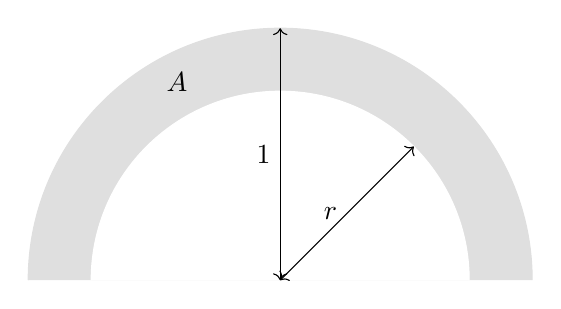
\begin{tikzpicture}[scale=0.8]
      % \draw[step=1cm, gray, very thin] (-4, -4) grid (4, 4);
      \draw[fill, gray!25] (4, -2) arc [start angle=0, end angle=180, radius=4cm];

      \draw[fill, white] (3, -2) arc [start angle=0, end angle=180, radius=3cm];

      \node[] at +(145:2) {$A$};
      \draw[<->] (0, -2) --+(45:3) node [midway, left] {$r$} ;
      \draw[<->] (0, -2) -- +(90:4) node [midway, left] {1} ;
    \end{tikzpicture}    
  }

  \bigskip
  \bigskip
  \[  
     \proba{x \in A} =\; \frac{vol(A)}{vol(\nball)}  =\; 1-r^n
   \]
\end{frame}


\begin{frame}{When is $x$ separable from the rest?}
  \twocols{
    \begin{itemize}
    \item {
        consider a hyperplane $H$ that is
        \begin{itemize}
        \item orthogonal to $x$
        \item and tangent to the inner ball $r \nball$
        \end{itemize}
      }
    \item $\allbutx$ are ``below'' $H$
    \item[] $\rightarrow$ $x$ is separable from $\allbutx$
    \item (the separating hyperplane is $H$)
    \end{itemize}
  }{
    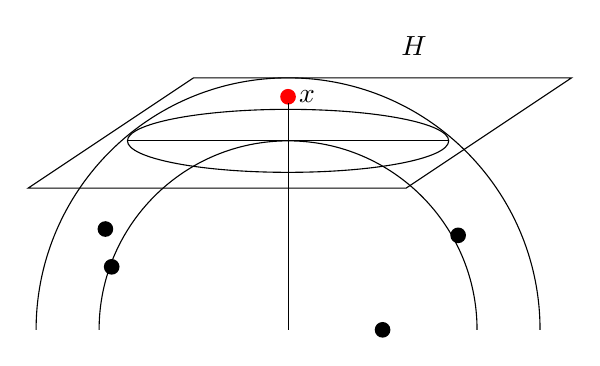
\begin{tikzpicture} [scale=0.8]
      % \draw[step=1cm, gray, very thin] (-4, -4) grid (4, 4);
      \draw (4, -2) arc [start angle=0, end angle=180, radius=4cm];

      \draw (3, -2) arc [start angle=0, end angle=180, radius=3cm];

      \node[] at (0.3, 1.7) {$x$};
      \node[fill=red, point] at (0, 1.7) {};

      \node[other point] at (-2.9, -0.4) {};
      \node[other point] at (-2.8, -1) {};
      \node[other point] at (1.5, -2) {};
      \node[other point] at (2.7, -0.5) {};

      % hyperplane
      \draw (0, -2) -- (0.0, 1.6);
      \pause
      \draw (0, 1) ellipse [x radius=2.55, y radius=0.5];
      \draw[xslant=1.5] (-4.5, 0.25) rectangle (1.5, 2);
      \draw (-2.55, 1) -- (2.55, 1);
      \node at (2, 2.5) {$H$};
    \end{tikzpicture}    
  }
  
  \[\proba{x \text{ is separable from } \allbutx} \ge \proba{\allbutx \text{ are below } H}\]

\end{frame}

\begin{frame}{what is $\proba{\allbutx \text{ are below } H}$?}

  \twocols{
    \begin{itemize}
    \item consider two points, $x$ and $v$
    \item analyze $\proba{v \text{ is above } H}$
    \item {then
        \begin{align*}
        & \proba{\allbutx \text{ are below } H} \\
        =\;& 1-\proba{ \exists v^{'} \in \allbutx \text{ is above } H} \\
        \ge\; &1 - \underbrace{\sum_{v^{'} \in \allbutx} \proba{v^{'} \text{ is above } H}}_{\text{by union bound}}
        \end{align*}

      }
    \end{itemize}
  }{
    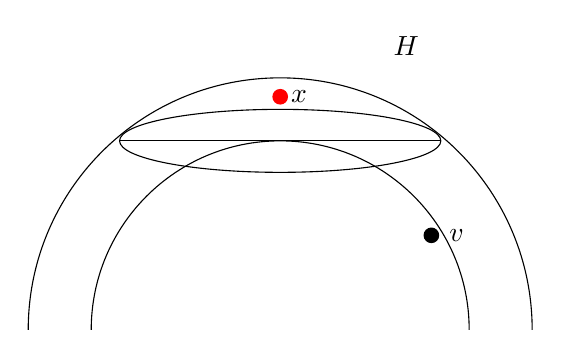
\begin{tikzpicture}[scale=0.8]
      % \draw[step=1cm, gray, very thin] (-4, -4) grid (4, 4);
      \draw (4, -2) arc [start angle=0, end angle=180, radius=4cm];
      \draw (3, -2) arc [start angle=0, end angle=180, radius=3cm];


      \node[] at (0.3, 1.7) {$x$};
      \node[fill=red, point] at (0, 1.7) {};
      \node[other point] at (2.4, -0.5) {};
      \node[] at (2.8, -0.5) {$v$};

      \draw (0, 1) ellipse [x radius=2.55, y radius=0.5];

      \node at (2, 2.5) {$H$};      
      \draw (-2.55, 1) -- (2.55, 1);

      % \draw (2.55, 1) arc [start angle=0, end angle=180, radius=2.55cm];
      
      % \draw[<->] (0, -2) --(2.55, 1) node [sloped, midway, below] {1} ;
      % \draw[<->] (0, -2) -- +(90:3) node [sloped, midway, below] {$r$} ;

      % \draw (0cm, 1cm) -- +(2.55, 0) node [sloped, midway, above] {$\sqrt{1-r^2}$} ;
      
    \end{tikzpicture}
  }
\end{frame}

\begin{frame}{Analysis of $\proba{v \text{ is above } H}$}
  \twocols{
    \begin{align*}
      & \proba{v \text{ is above } H} \\
      =\;& \proba{v \text{ lands in  "the cap"}} \\
      =\;& \frac{vol(\text{"the cap"})}{vol(\nball)} \\
      \le \;& \frac{vol(\text{"half the ball"})}{vol(\nball)} \\
      = \;& 0.5 \rho^n
    \end{align*}
    Radius of the ball? $\rightarrow \sqrt{1 - r^2} = \rho$
  }{
    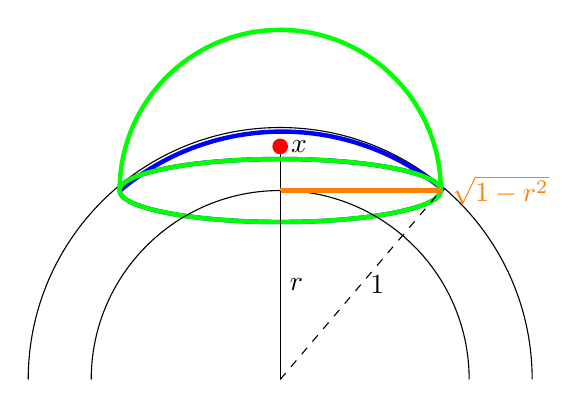
\begin{tikzpicture}[scale=0.8]
      % \draw[step=1cm, gray, very thin] (-4, -4) grid (4, 4);
      \draw (4, -2) arc [start angle=0, end angle=180, radius=4cm];


      \node[] at (0.3, 1.7) {$x$};
      \draw (0, -2) -- (0, 1.7);
      \node[fill=red, point] at (0, 1.7) {};
      
      % \node[other point] at (2.4, -0.5) {};
      % \node[] at (2.8, -0.5) {$v$};

      % \draw[dashed] (2.4, -0.5) -- (0, -0.5);
      % \draw[ultra thick, blue] (0, -2) -- (0, -0.5);


      \only<1>{
        \draw[blue, ultra thick] (0, 1) ellipse [x radius=2.55, y radius=0.5];
        \draw[blue, ultra thick] (2.6, 1) arc [start angle=50, end angle=130, radius=4cm];
      }

      % \node at (2, 2.5) {$H$};

      \uncover<2->{
      % \draw (-2.55, 1) -- (2.55, 1);
      \draw[green, ultra thick] (2.55, 1) arc [start angle=0, end angle=180, radius=2.55cm];
      \draw[green, ultra thick] (0, 1) ellipse [x radius=2.55, y radius=0.5];
      % \draw[<->] (0, -2) --(2.55, 1) node [sloped, midway, below] {1} ;
      % \draw[<->] (0, -2) -- +(90:3) node [sloped, midway, below] {$r$} ;
    }
    \uncover<3->{
      \draw (3, -2) arc [start angle=0, end angle=180, radius=3cm];
      \draw[ultra thick, orange] (0cm, 1cm) -- +(2.55, 0) node [sloped, right] {$\sqrt{1-r^2}$} ;
      \draw[dashed] (0, -2) -- (2.55, 1) node [right, midway] {$1$};
      \draw (0, -2) -- (0, 1) node [right, midway] {$r$};
    }
    \end{tikzpicture}
  }
\end{frame}

\begin{frame}{Putting things together}
  \begin{align*}
    & \proba{x \text{ is separable from } \allbutx} \\
    \ge\;&\proba{x \in A \text{ and } \allbutx \text{ are below } H} \\
    \ge\;& 1 - \underbrace{\proba{x \not\in A}}_{r^n} - \underbrace{\proba{\exists v^{'} \in \allbutx \text{ that is above } H}}_{\le \sum_{v^{'} \in \allbutx} \underbrace{\proba{v^{'} \text{ is above }H}}_{\le \rho^n}} \\
    \ge\; & 1 - r^n - \pr{M-1} \rho^n
  \end{align*}
\end{frame}

\begin{frame}{}
  \begin{center}
    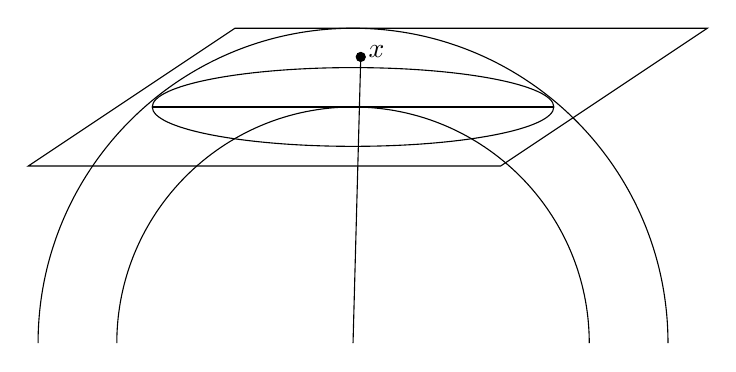
\begin{tikzpicture}
      % \draw[step=1cm, gray, very thin] (-4, -4) grid (4, 4);
      \draw (4, -2) arc [start angle=0, end angle=180, radius=4cm];

      \draw (3, -2) arc [start angle=0, end angle=180, radius=3cm];
      \draw[-Circle] (0, -2) -- (0.1, 1.7) node[xshift=0.2cm] {$x$};  % circle requires loading arrows.meta
      % \node[] at (0.1, 1.7) {$x$};

      \draw (0, 1) ellipse [x radius=2.55, y radius=0.5];

      \draw[xslant=1.5] (-4.5, 0.25) rectangle (1.5, 2);
      \draw (-2.55, 1) -- (2.55, 1);

      % \draw (2.55, 1) arc [start angle=0, end angle=180, radius=2.55cm];
      
      % \draw[<->] (0, -2) --(2.55, 1) node [sloped, midway, below] {1} ;
      % \draw[<->] (0, -2) -- +(90:3) node [sloped, midway, below] {$r$} ;

      % \draw (0cm, 1cm) -- +(2.55, 0) node [sloped, midway, above] {$\sqrt{1-r^2}$} ;
    \end{tikzpicture}
  \end{center}

\end{frame}

\begin{frame}{}
  \centering
  {\Large separating two sets of points}

  \begin{tikzpicture}
    % \draw (-2, -2) grid (2, 2);
    

      \node[fill=red, point] at (150:2) {};
      \node[fill=red,  point] at (120:2) {};
      \node[fill=blue, point] at (-30:1.5) {};
      \node[fill=blue, point] at (45:2) {};
      \node[fill=blue, point] at (-90:0.5) {};


      \draw[thick, gray, dashed] (-1.7, -1.7) -- (.5, 2);

  \end{tikzpicture}
\end{frame}

\begin{frame}{setting}
  \twocols{
    \begin{itemize}
    \item given a set of points $\allpts \in \rn$
    \item \uncover<2->{a dichotomy $\bipart$ of $\allpts$ is \textit{homogeneously linearly separable} }
    \item \uncover<3->{iff there is a vector $w \in \rn$  s.t.
        \begin{align*}
          x \cdot w > 0 & \text{ if } x\in\Xpos\\
          x \cdot w < 0 & \text{ if } x\in\Xneg\\
        \end{align*}
      }
    \item \uncover<3->{the separating hyperplane is the $(d-1)$ orthogonal subspace to $w$}
    \item \uncover<4->{the hyperplane must pass through the origin}
    \end{itemize}
  }{
    \centering
    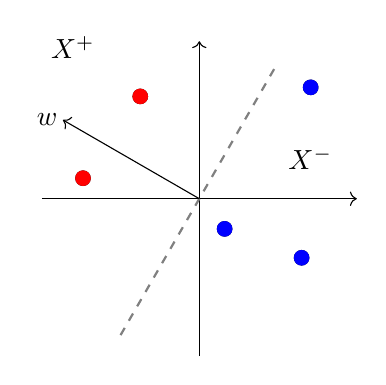
\begin{tikzpicture}      
      \draw[->] (-2, 0) -- (2, 0);
      \draw[->] (0, -2) -- (0, 2);

      \uncover<1>{
        \node[other point] at (170:1.5) {};
        \node[other point] at (120:1.5) {};
        \node[other point] at (-30:1.5) {};
        \node[other point] at (45:2) {};
        \node[other point] at (-50:0.5) {};
      }
      
      \uncover<2->{
        \node[fill=red, point] at (170:1.5) {};
        \node[fill=red,  point] at (120:1.5) {};
        \node[fill=blue, point] at (-30:1.5) {};
        \node[fill=blue, point] at (45:2) {};
        \node[fill=blue, point] at (-50:0.5) {};
        \node at (130:2.5) {$\Xpos$};
        \node at (20:1.5) {$\Xneg$};        
      }
      \uncover<3->{
        \draw[thick, gray, dashed] (-120:2) -- (60:2);
        \draw[->] (0, 0) -- (150:2) node[xshift=-0.2cm] {$w$};
      }
      
    \end{tikzpicture}

    \uncover<4>{two separable dichotomies
      
    $\pr{\set{\text{\tikz\node[point, fill=blue] at (0, 0) {};}}, \set{\text{\tikz\node[point, fill=red] at (0, 0) {};}}}$
    and $\pr{\set{\text{\tikz\node[point, fill=red] at (0, 0) {};}}, \set{\text{\tikz\node[point, fill=blue] at (0, 0) {};}}}$}
  }
\end{frame}

\newcommandx*{\warmupone}[4][1=black, 2=black, 3=black, 4=]{
    \begin{tikzpicture}[scale=0.8]
      \draw[gray!20] (-2, 0) -- (2, 0);
      \draw[gray!20] (0, -2) -- (0, 2);

      \node[fill=#1, point] at (90:1.5) {};
      \node[fill=#2, point] at (-30:1.5) {};
      \node[fill=#3, point] at (210:1.5) {};
   
      % \draw[thick, gray, dashed] (-120:2) -- (60:2);
      #4
    \end{tikzpicture}
  
}
\begin{frame}{warm-up 1/2}
  how many separable dichotomies?

  \begin{tabular}{cccc}
    \warmupone
    &   \uncover<2->{\warmupone[blue][red][red][{\draw[thick, gray, dashed] (180:2) -- (0:2);}]}
    & \uncover<3->{\warmupone[red][blue][red][{\draw[thick, gray, dashed] (-135:2) -- (45:2);}]}
    & \uncover<4->{\warmupone[red][red][blue][{\draw[thick, gray, dashed] (135:2) -- (-45:2);}]} \\
    & \uncover<2->{2} & \uncover<3->{+\; 2} & \uncover<4->{+\;2} \\
    & & & \\
    &  & \uncover<5->{=\; 6} & 
  \end{tabular}
\end{frame}

\newcommandx*{\warmuptwo}[3][1=black, 2=black]{
  \begin{tikzpicture}[scale=0.8]
    \draw[gray!20] (-2, 0) -- (2, 0);
    \draw[gray!20] (0, -2) -- (0, 2);

    \node[fill=#1, point] at (170:1.5) {};
    \node[fill=#2, point] at (270:1) {};
    \node[fill=#2, point] at (270:2) {};
    
    % \draw[thick, gray, dashed] (-120:2) -- (60:2);
    #3
  \end{tikzpicture}  
}

\begin{frame}{warm-up 2/2}
  how many separable dichotomies?

  \centering
  \begin{tabular}{ccc}
    \warmuptwo{}  &
    \uncover<2->{\warmuptwo[red][blue]{{\draw[thick, gray, dashed] (-135:2) -- (45:2);}}} & \uncover<3->{\warmuptwo[red][red]{{\draw[thick, gray, dashed] (135:2) -- (-45:2);}}}\\
                & \uncover<2->{2} & \uncover<3->{+\; 2} \\
                & & \uncover<4->{=\; 4} \\
  \end{tabular}

  \bigskip

  \uncover<5->{Fewer than the previous example. }
\end{frame}

\begin{frame}{assumption: points are in general position}
  \twocols{
    Why 4 not 6?\pause
    \bigskip
    
    \warmuptwo[black][orange]{
      \draw[orange, dashed] (0, -1.5) circle [radius=1];
      \node[text width=4cm] at (4, -3) {linearly dependent \\$\Rightarrow$ \textbf{inseparable} \\(by any hyperplane through origin)};
    }    
  }{
    \pause
     $\allpts$ are in \textit{general position} if

    \begin{itemize}
    \item every subset of size $d$ or fewer are \textit{linearly independent}
    \end{itemize}

    \pause
    Why assuming so?
    \pause
    \begin{itemize}
    \item we can analyze the \textbf{upper bound} on the number of separable dichotomies
    \item points are likely to be in general position (e.g., if points are uniformly distributed)
    \end{itemize}
    
  }

\end{frame}

\begin{frame}{main character -- $C(N, d)$}
  \centering
  {\large
    \[
      C(N, d) = \text{\# of linearly separable dichotomies of } N \text{ in } \mathbb{R}^d
    \]

    \pause
    \hfill \txtgray{(assuming $\allpts$ in general position )}
    \bigskip

    \pause
    \head{Question}: does $C(N, d)$ have a closed-form formula?
  }
\end{frame}

\newcommand{\proofviz}[1]{
  \begin{tikzpicture}      
    \draw[gray!20] (-2, 0) -- (2, 0);
    \draw[gray!20] (0, -2) -- (0, 2);

    \node[other point] at (170:1.5) {};
    \node[other point] at (120:1.5) {};
    \node[other point] at (-30:1.5) {};
    \node[other point] at (40:2) {};
    \node[other point] at (-50:0.5) {};

    \draw[thick, gray, dashed] (-120:2) -- (60:2);
    % \draw[->] (0, 0) -- (150:2) node[xshift=-0.2cm] {$w$};
    
    \node at (130:2.5) {$\Xpos$};
    \node at (20:1.5) {$\Xneg$};

    #1
  \end{tikzpicture}    
}
\begin{frame}{analysis by induction 1/6}
  \begin{itemize}[<+->]
  \item assume we have $N$ points $\allpts$ and add a new point $y$
  \item for each separable $\bipart$ of $\allpts$, there are two possibilities of $y$, depending on
  \item if there is a separating hyperplane $w$ of $\bipart$ s.t. $w\cdot y = 0$
  \end{itemize}

  \centering
  \begin{tabular}{cc}
    \setlength\tabcolsep{50pt}
    \uncover<4->{case 1: \txtred{no}} & \uncover<5->{case 2: \txtdgreen{yes}} \\
    \uncover<4->{\proofviz{{\node[point, fill=red] at (130:2) {};}}} &
    \uncover<5->{\proofviz{{\node[point, fill=red] at (60:0.6) {};}}} \\
  \end{tabular}

\end{frame}

\begin{frame}{analysis by induction 2/6}
  \head{case 1}
  
  \begin{itemize}
  \item i.e., there is \textbf{no} such separating hyperplane $w$ s.t. $w\cdot y = 0$\pause
  \item either $\pr{\Xpos \cup \set{y}, \Xneg}$ or $\pr{\Xpos, \Xneg  \cup \set{y}}$ is separable
  \item \uncover<3>{$\Rightarrow$ \txtred{1} separable dichotomy for $\allpts \cup \set{y}$.}
  \end{itemize}

  \centering
  \proofviz{{\node[point, fill=red] at (130:2) {};}}
\end{frame}


\begin{frame}{analysis by induction 3/6}
  \head{case 2}
  
  \begin{itemize}
  \item i.e., there is such separating hyperplane $w$ s.t. $w\cdot y = 0$\pause
  \item  \textbf{both} $\pr{\Xpos \cup \set{y}, \Xneg}$ and $\pr{\Xpos, \Xneg  \cup \set{y}}$ are separable
  \item \uncover<5>{$\Rightarrow$ \txtred{2} separable dichotomies for $\allpts \cup \set{y}$.}
  \end{itemize}

  \centering
  \proofviz{
      \node[point, fill=red] at (60:0.6) {};

    \only<3, 5>{
      % \draw[thick, white, dashed] (-120:2) -- (60:2);  % over the HP
      % \node[point, fill=red!20] at (88:0.4) {};
      \draw[ultra thick, blue, dashed] (-100:2) -- (80:2);
    }

    \only<4, 5>{
      % \draw[thick, white, dashed] (-120:2) -- (60:2);  % over the HP
      % \node[point, fill=red!20] at (30:0.4) {};
      \draw[ultra thick, blue, dashed] (-135:2) -- (45:2);
    }
  }
\end{frame}

\begin{frame}{analysis 4/6: combining case 1 and case 2}
  \begin{itemize}
  \item let $D$ be the number of ``case-2'' dichotomies. \pause
  \item[] {
      \begin{align*}
        C(N+1, d) &= \underbrace{C(N, d) - D}_{1\times\text{\# of case 1 dich.}} + \underbrace{2\;D}_{2\times \text{\# of case 2 dich.}}\\
                  &= C(N, d) + D
      \end{align*}
      
    }\pause
    \item \head{question}: what is $D$?
  \end{itemize}
  


\end{frame}

\begin{frame}{analysis 5/6: what is $D$?}
  recall $D$ is the number of $\bipart$ for which there is a separating $w$ s.t. $w\cdot y = 0$.

  \begin{minipage}{0.68\textwidth}
    \uncover<2->{
    \begin{lemma}
      $\pr{\Xpos \cup \set{y}, \Xneg}$ and $\pr{\Xpos, \Xneg  \cup \set{y}}$ are both separable in $\mathbb{R}^d$
      \begin{center}
        $\Leftrightarrow$
      \end{center}

      $\bipart$ is separable by a $(d-1)$-dimensional space containing $y$
    \end{lemma}
  }
    \bigskip
    \uncover<3>{
      $\Rightarrow D\;=\;C(N, d-1)$ $\quad \leftarrow$ \head{the key!}
    }
  \end{minipage}
  \begin{minipage}{0.3\textwidth}
    \centering
    \proofviz{
      \node[point, fill=red] at (60:0.6) {};
    }
  \end{minipage}      
\end{frame}


\begin{frame}{proof of lemma 1/2}
      $\pr{\Xpos \cup \set{y}, \Xneg}$ and $\pr{\Xpos, \Xneg  \cup \set{y}}$ are separable   \txtblue{$\Leftarrow$} $\bipart$ is separable by a $(d-1)$-dimensional space containing $y$

    \uncover<3->{
      Simple, recall that the hyperplane can be shifted either way
    }
    \uncover<2->{
      \begin{center}
        \proofviz{
          \node[point, fill=red] at (60:0.6) {};
          \draw[ultra thick, blue, dashed] (-100:2) -- (80:2);    
          \draw[ultra thick, blue, dashed] (-135:2) -- (45:2);          
        }
      \end{center}
    }

\end{frame}

\begin{frame}{proof of lemma 2/2}
      $\pr{\Xpos \cup \set{y}, \Xneg}$ and $\pr{\Xpos, \Xneg  \cup \set{y}}$ are separable   \txtblue{$\Rightarrow$} $\bipart$ is separable by a $(d-1)$-dimensional space containing $y$
\pause
\begin{itemize}[<+->]
	\item {let $w_1$ by a hyperplane that separates $\pr{\Xpos \cup \set{y}, \Xneg}$
	\begin{itemize}
		\item $w_1 \cdot y > 0$
	\end{itemize}
	}
	\item {let $w_2$ by a hyperplane that separates $\pr{\Xpos, \Xneg \cup \set{y}}$
		\begin{itemize}
		\item $w_2 \cdot y < 0$
	\end{itemize}
	}
	\item let $w^* = (-w_2 \cdot y) w_1 + (w_1 \cdot y) w_2$
	\item \head{fact 1}: $w^* \cdot y = 0$ 
	\item[]  $\quad\rightarrow\quad$ $y$ is contained by the hyperplane $w^*$
        \item[] $\quad\rightarrow\quad$ what is this hyperplane? \pause the subspace orthogonal to $y$!
	\item \head{fact 2}: $w^*\cdot x  > 0$ for $x \in \Xpos$ and  $w^* \cdot x  < 0$ for $x \in \Xneg$ 
	\item[] $\quad \rightarrow \quad$ $\bipart$ is separated by $w^*$
\end{itemize}
\end{frame}

\begin{frame}{analysis 6/6}
  \begin{align*}
    C(N, d) &= C(N-1, d) + \txtblue{C(N-1, d-1)} \\
            & \ldots\ldots \text{ expand recursively } \ldots\ldots \\
            &=  \sum\limits_{k=0}^{N-1} {N -1\choose k} C(1, d-k)
  \end{align*}

  \pause
  note that:
  $$
    C(1, m) = 
    \begin{cases}
      2, &m \ge 1 \\
      0, &m < 1
    \end{cases}
    $$

    \pause
\[
  \Rightarrow \quad C(N, d) = 2\;\sum\limits_{k=0}^{d-1} {N -1\choose k} \quad \longleftarrow \quad \text{\head{Cover's theorem}}
\]

\end{frame}

\begin{frame}{verify it!}

\begin{itemize}
\item $C(N, d) =  \sum\limits_{k=0}^{N-1} {N -1\choose k} C(1, d-k)$
\item \uncover<4>{$C(3, 2) =   {2\choose 1} C(1, 1) + {2\choose 0} C(1, 2) = 3 \times 2 = 6$}
\item \uncover<6>{$C(4, 2) =   {3\choose 1} C(1, 1) + {3\choose 0} C(1, 2) = 4 \times 2 = 8$}
\end{itemize}

  \begin{tabular}{ccc}
    \uncover<2,4>{$d=2, N=3$} & \uncover<3,4>{$d=2, N=3$} &  \uncover<5,6>{$d=2, N=4$} \\
    \uncover<2,4>{
    \begin{tikzpicture}      
      \draw[gray!20] (-2, 0) -- (2, 0);
      \draw[gray!20] (0, -2) -- (0, 2);

      \node[other point] at (170:1.5) {};
      \node[other point] at (120:1.5) {};
      \node[other point] at (-30:1.5) {};
    \end{tikzpicture}}    &
\uncover<3,4>{                            
\begin{tikzpicture}      
    \draw[gray!20] (-2, 0) -- (2, 0);
    \draw[gray!20] (0, -2) -- (0, 2);

    \node[other point] at (170:1.5) {};
    \node[other point] at (120:1.5) {};
    \node[other point] at (150:1) {};
  \end{tikzpicture}}             &
\uncover<5,6>{
\begin{tikzpicture}      
    \draw[gray!20] (-2, 0) -- (2, 0);
    \draw[gray!20] (0, -2) -- (0, 2);

    \node[other point] at (170:1.5) {};
    \node[other point] at (120:1.5) {};
    \node[other point] at (-15:1.5) {};
    \node[other point] at (45:1.5) {};
  \end{tikzpicture}
}
  \end{tabular}
\end{frame}

\begin{frame}{generalization of Cover's theorem}
  \begin{theorem}
    if the hyperplane is constrained to contain $k$ linearly independent points $\set{y_1, \ldots, y_k}$, then there are $C(N, d-k)$ separable dichotomies of $\allpts$. 
  \end{theorem}
  \pause
  \txtblue{an assumption}: projection of \allpts onto the orthogonal subspace of $S(\set{y_1, \ldots, y_k})$ are in general position, where $S(\set{\cdot})$ is the space spanned by $\set{\cdot}$.
\end{frame}

\begin{frame}{generalization to arbitrary surfaces}
  \begin{itemize}[<+->]
  \item say $\allpts$ are in $\Rm$, for now, we only considered \textit{linear separability} in $\Rm$.
  \item {what if $\allpts$ are not linearly separable in $\Rm$?

      \begin{center}
        \begin{tikzpicture}[scale=0.8]

          \draw[gray!50, ->] (-4, 0) -- (4, 0);
          \draw[gray!50, ->] (0, -1) -- (0, 1);

          \node[point, fill=red] at (1.5, -0.3) {};
          \node[point, fill=red] at (-1.5, 0.2) {};
          \node[point, fill=blue] at (3, 0.3) {};
          \node[point, fill=blue] at (-3, -0.2) {};
        \end{tikzpicture}
      \end{center}

    }
  \item {can we transform them into  \textit{a higher-dimensional space} $\rd$ so that they \textit{are} linearly separable?}
  \item {the separating surface in \Rm is possibly \textit{non-linear}.
      \begin{center}
        \begin{tikzpicture}[scale=0.8]

          \draw[gray!50, ->] (-4, 0) -- (4, 0);
          \draw[gray!50, ->] (0, -1) -- (0, 1);

          \node[point, fill=red] at (1.5, -0.3) {};
          \node[point, fill=red] at (-1.5, 0.2) {};
          \node[point, fill=blue] at (3, 0.3) {};
          \node[point, fill=blue] at (-3, -0.2) {};

          \draw[dashed, orange, thick] (0, 0) circle [radius=2cm];
        \end{tikzpicture}
      \end{center}
    }
  \end{itemize}
\end{frame}

\begin{frame}{generalization to arbitrary surfaces}
  \begin{itemize}
  \item assume each point $x \in \mathbb{R}^m$ is transformed into  $\mathbb{R}^d$ where $d > m$
  \item by some function $\phi: \mathbb{R}^m \rightarrow \mathbb{R}^d$
  % \item if $\allpts$ are not linearly separable in $\mathbb{R}^m$
  % \item can we separate \allpts linearly in the new space $\mathbb{R}^d$?		
  \end{itemize}
\end{frame}

\begin{frame}{arbitrary surface examples 1/2}

  \twocols{
    \centering

    \begin{tikzpicture}[scale=0.8]

      \draw[gray!50, ->] (-1, 0) -- (4, 0);
      \draw[gray!50, ->] (0, -1) -- (0, 1);

      \node[point, fill=red] at (1, 0.4) {};
      \node[point, fill=red] at (2, 0) {};
      \node[point, fill=blue] at (3, -0.8) {};

      \uncover<2->{
        \draw[dashed, orange, thick] (2.5, -2) -- (2.5, 2);
      }
    \end{tikzpicture}

    What if $\phi(x) = (1, x)$?

    \uncover<2->{
      $\Rightarrow$

      separating surfaces = \head{hyperplanes not necessarily passing through origin}
      
      \bigskip
      
      degree of freedom: $d+1$
    }
  }{
    \centering
    \begin{tikzpicture}[scale=0.8]

      \uncover<3->{      
        \draw[gray!50, ->] (-4, 0) -- (4, 0);
        \draw[gray!50, ->] (0, -1) -- (0, 1);

          \node[point, fill=red] at (1.5, -0.3) {};
          \node[point, fill=red] at (-1.5, 0.2) {};
          \node[point, fill=blue] at (3, 0.3) {};
          \node[point, fill=blue] at (-3, -0.2) {};
      }
      \uncover<4->{      
        \draw[dashed, orange, thick] (0, 0) circle [radius=2cm];
      }
    \end{tikzpicture}

    \uncover<3->{    
      What if $\phi(x) = (1, x, ||x||^2)$?

    }
    \uncover<4->{
      $\Rightarrow$

      separating surfaces = \head{hyperspheres}
      
      \bigskip
      
      degree of freedom: $d+2$
      
    }
  }
\end{frame}

\begin{frame}{arbitrary surface examples 2/2}
	\begin{itemize}
		\item let $\phi$ be all $r$-wise products of $x_i$
		\item i.e., $\phi(x)=\pr{1, x_1, x_2, \ldots, x_m, (x_1)^2, x_1 x_2, \ldots, x_i x_j, \ldots, x_m^r}$ \pause
                \item the surface is called a rational $r$th-order variety\pause
                \item degree of freedom: ${m+r \choose r}$
	\end{itemize}
\end{frame}

\begin{frame}{generalization to arbitrary surfaces: a summary}
	\resizebox{\columnwidth}{!}{%
	\begin{tabular}{c|c|c|m{3cm}|c} %{m{2cm}|m{4cm}|m{2cm}|m{3cm}|m{2cm}}
	def. of $\phi(x)$ & separating surface & degree of freedom & number of separable dichotomies & separating capacity \\	\hline
	$(x)$ & hyperplane through origin & $m$ & $C(N, m)$ & $2m$ \\
	$(1, x)$ & hyperplane & $m+1$ & $C(N, m+1)$ & $2\pr{m+1}$ \\
	$(1, x, ||x||_2)$ & hypersphere& $m+2$ & $C(N, m+2)$ & $2\pr{m+2}$ \\
	$( x, ||x||_2)$ & hypercone& $m+1$ & $C(N, m+1)$ & $2\pr{m+1}$ \\
	$\text{all $r$-wise products of $x_i$}$ & rational $r$-order variety& ${m+r \choose r}$ & $C(N, {m+r \choose r})$ & $2\pr{{m+r \choose r}}$ \\	
	\end{tabular}
	}
\end{frame}


\begin{frame}{}
  \centering
  {\large let's go back to $\rd$ and consider linear separability again.}
\end{frame}
  
\begin{frame}{probability of being separable}
  \begin{itemize}
  \item let $P(N, d)$ be the probability of a random dichotomy being linearly separable\pause
  \item further assume each dichotomy has equal chance of being drawn\pause $\rightarrow 1/2^N$\pause
  \item[] {
      \begin{align*}
        P(N, d) &= \sum_{\bipart} \pr{\frac{1}{2}}^N \indicator{\bipart \text{ is separable}} \\
                &=\pr{\frac{1}{2}}^N C(N, d) \\
                &= \pr{\frac{1}{2}}^{N-1} \sum\limits_{k=0}^{d-1} {N-1 \choose k}
      \end{align*}\pause
    }
  \item What is $P(N, d)$?\pause
  \item $\Rightarrow$ cumulative binomial distribution
  \item[] i.e., $N-1$ flips of a fair coin resulting in $d-1$ or fewer heads.
  \end{itemize}
\end{frame}

\begin{frame}{What does $P(N, d)$ look like?}
 \begin{center}
   \includegraphics[width=0.8\textwidth]{images/pnd}
 \end{center}
\end{frame}

\begin{frame}{}
  \begin{center}
    {\large
      \txtblue{how many points} can a $d$-dimensional space naturally have

      s.t. $P(N, d)$ is \txtblue{high}?

    \bigskip
    
    $\Rightarrow$ \head{separating capacity}
  }
  \end{center}
\end{frame}

\begin{frame}{separating capacity 1/2}  
  \begin{itemize}
  \item[] {
      \begin{center}
        \includegraphics[width=0.5\textwidth]{images/pnd-n}
      \end{center}
    }\pause    
  \item {
      given some integer $n$, consider 
      
      \[
        P(n, d) - P(n+1, d) = \halfn {n-1 \choose d-1}
      \]
    }
  \item \pause interpretation: speed of change w.r.t. $n$ at $n$ ("derivative")
  \item \pause$\rightarrow\quad$negative binomial distribution!
  \end{itemize}
\end{frame}
	
\begin{frame}{Separating capacity 2/2}
	\begin{itemize}	
		\item {asymptotic behaviour, for $\epsilon > 0$\pause
		\begin{align*}
		\lim\limits_{d \rightarrow \infty} P(2d(1+\epsilon), d) &= 0 \\
		\lim\limits_{d \rightarrow \infty} P(2d, d) &= \half \\
		\lim\limits_{d \rightarrow \infty} P(2d(1+\epsilon), d) &= 1 \\
		\end{align*}\pause
		\item $2d$ is the \textbf{separating capacity} of a surface family having $d$ \textit{degrees of freedom}.
		}
	\end{itemize}
\end{frame}


\sectionslide{Implications on classification -- generalization and learning}

\begin{frame}{generalization and learning: setting}
\begin{itemize}[<+->]
	\item assume we have a \head{binary classification problem}
	\item with training set $\bipart$
	\item a new point $y$ is said to be \head{ambiguous} w.r.t. a family of surfaces
	\item if there exists one surface inducing the dichotomy \txtblue{$\pr{\Xpos \cup \set{y}, \Xneg}$}
	\item and there exists another surface inducing the dichotomy \txtred{$\pr{\Xpos, \Xneg  \cup \set{y}}$}
\end{itemize}

\bigskip
\pause
\centering\large two classifiers trained on $\bipart$ give \head{different predictions} on $y$.
\end{frame}

\begin{frame}{an example of being ambiguous}
  \centering
  \begin{tikzpicture}
    % \draw[help lines, gray] (-4, -4) grid (4, 4);
    \node[] at (-3.5, 3.5) {$X^{+}$};
    \draw[] (-2, 1) node[point, fill=red] {} -- (0, 2) node[point, fill=red] {} -- (-3, 3) node[point, fill=red] {} -- cycle;
    
    \draw[] (-3, -1) node[point, fill=blue] {} -- (1, -0.5) node[point, fill=blue] {} -- (0, -3) node[point, fill=blue] {} -- cycle;
    
    \draw[ fill=gray] (1.2, -3) circle (2pt) node[anchor=west] {$y_1$};
    \draw[ fill=gray] (1.5, 0.5) circle (2pt) node[anchor=west] {$y_2$};
    \draw[ fill=gray] (1, 3) circle (2pt) node[anchor=west] {$y_3$};
    
    \draw[gray](-3,-0.5) -- (3, 2) node [black, anchor=west] {$\ell_1$};
    \draw[gray](-3, 0) -- (3, 0) node [black, anchor=west] {$\ell_2$};
  \end{tikzpicture}
\end{frame}


\begin{frame}{condition of ambiguity}
  \begin{itemize}
  \item when is $y$ ambiguous?
  \item {
      \uncover<3>{when there exists a separating surface \txtblue{containing} $y$!}

      \uncover<2->{
        \begin{center}
          \proofviz{
            \node[point, fill=red] at (60:0.6) {};
          }   
        \end{center}
      }
    }
  \end{itemize} 
\end{frame}

\begin{frame}{probability of ambiguity}
  \begin{itemize}[<+->]
  \item what is the probability that $y$ is ambiguous, given a training set of $N$ points in $\mathbb{R}^d$?
  \item let $A(N, d)$ denote this probability 
  \item[] {
      \begin{align*}
        A(N, d) &=\; \frac{\text{\# of separable dich. containing } y}{\text{\# of separable dich.}}\\
                &=\; \frac{C(N, d-1)}{C(N, d)}
      \end{align*}
    }
  \end{itemize}
\end{frame}

\begin{frame}{asymptotic behaviour of  $A(N, d)$)}
  \twocols{
    \begin{itemize}
    \item let $\beta=\frac{N}{d}$
    \item {let $A^{*}(\beta) = \lim\limits_{N = \beta d, d\rightarrow \infty} A(N, d)$}
    \item{(after some analysis)
        \[
          A^{*}(\beta) = 
          \begin{cases}
            1, & 0 \le \beta \le 2 \\
            \frac{1}{\beta-1} & \beta \ge 2
          \end{cases}
        \]
      }
    \end{itemize}
  }{
    \pause
    \centering
    \includegraphics[width=1\textwidth]{images/Abeta}
  }
\end{frame}

\begin{frame}{Implications}
\begin{itemize}[<+->]
	\item more data $\quad\Rightarrow\quad$ less ambiguity
	\item one manifestation of ``curse of dimensionality''
        \item[] as $d \uparrow$, more data is need to \textit{generalize unambiguously}
	\item[] {
	\centering
	\bigskip
	\includegraphics[width=0.8\textwidth]{images/andrew-ng}~\footnote{https://analyticsindiamag.com/big-data-to-good-data-andrew-ng-urges-ml-community-to-be-more-data-centric-and-less-model-centric/}
	}
\end{itemize}
\end{frame}

\begin{frame}{summary}
  \begin{itemize}[<+->]
  \item {Cover's theorem (proved by induction):
      \[
        C(N, d) = 2\;\sum\limits_{k=0}^{d-1} {N -1\choose k}
      \]
    }
  \item separating capacity of a family of surfaces having $d$ degree of freedom $\Rightarrow$ $2d$
  \item {implications
      \begin{itemize}
      \item transforming data into a higher-dimensional space $\rightarrow$ linear separability (kernel SVM, neural networks, etc)
      \item the need for more data for classifiers to generalize unambiguously
      \item more?
      \end{itemize}
    }
  \end{itemize}
\end{frame}

\begin{frame}{reference}
  \begin{centering}
    {\large
      Cover, Thomas M. ``Geometrical and statistical properties of systems of linear inequalities with applications in pattern recognition.'' \textit{IEEE transactions on electronic computers} (1965)
    }
  \end{centering}
\end{frame}

\end{document}


